\documentclass[11pt]{article}
\usepackage[a4paper,margin=1in]{geometry}
\usepackage[T1]{fontenc}
\usepackage[utf8]{inputenc}
\usepackage{lmodern}
\usepackage{microtype}
\usepackage{setspace}
\usepackage{graphicx}
\usepackage{booktabs}
\usepackage{enumitem}
\usepackage{hyperref}
\usepackage{float}
\usepackage[numbers,sort&compress]{natbib}

\setlength{\parskip}{0.5em}
\setlength{\parindent}{0pt}

\title{BABAPPASNAKE: A Workflow for Episodic Selection Analysis with Robustness-Aware Summaries and an Empirical Demonstration in Mosquito Melanization Genes}
\author{Krishnendu Sinha}
\date{}

\begin{document}
\maketitle

\begin{abstract}
Episodic selection studies are often assembled from multiple disconnected tools, and practical reproducibility is frequently limited by alignment choices, trimming choices, and ad hoc decision logic across analysis stages.
We present \textbf{BABAPPASNAKE}, an integrated workflow for orthogroup-centered episodic selection analysis.
The workflow combines orthogroup definition, CDS quality control and mapping, multi-engine alignment pathways, phylogenetic inference, exploratory nomination, branch-site follow-up testing, and structured reporting in a single executable framework.
BABAPPASNAKE produces pathway-specific and cross-pathway robustness outputs (including matrix, consensus, narrative, provenance, and archival summaries) to support sensitivity-aware interpretation rather than single-path overinterpretation.
We use a four-gene mosquito melanization-associated analysis as an empirical end-to-end demonstration of workflow behavior on real data.
Across this demonstration, BABAPPASNAKE exposes both recurrent and method-sensitive signals, including pathway-dependent differences in reproducibility classes.
These observations are presented as directional and hypothesis-generating patterns rather than decisive pathway-level proof.
Overall, BABAPPASNAKE provides a practical and reproducible framework for episodic selection workflows where analytical sensitivity must be made explicit.
\end{abstract}

\section{Introduction}
Episodic selection inference is widely used in evolutionary genomics, but practical implementation remains fragmented.
Typical analyses combine ortholog collection, codon-aware alignment, tree estimation, exploratory scans, branch-targeted confirmatory tests, and post hoc reporting through separate scripts and tools.
In this setting, scientific interpretation can be dominated by implementation details that are not consistently tracked, and reproducibility can be weakened by undocumented analyst decisions.

A central practical challenge is sensitivity to workflow choices.
Orthogroup construction strategy, alignment engine, trimming behavior, branch selection rules, and model-parameter settings can all alter which signals are retained, attenuated, or lost.
Without explicit cross-path reporting, users may unintentionally treat one analytical route as definitive.

BABAPPASNAKE was developed to address this implementation gap as a workflow contribution.
The goal is not to replace established inference engines, but to orchestrate them reproducibly and to report robustness structure explicitly.
The workflow is implemented with Snakemake and integrates major stages of orthogroup-centered episodic selection analysis into one resumable execution model \citep{snakemake2012,babappasnake_repo}.

To demonstrate practical utility on real data, we use a mosquito melanization-associated four-gene module as an empirical case study.
This biological system is used here as a realistic workflow showcase, not as the sole basis for broad biological claims.

\textbf{Contribution statement.}
This study introduces BABAPPASNAKE as a robustness-aware episodic selection workflow and demonstrates its practical use on a mosquito melanization-associated gene module.

\section{Workflow Design and Implementation}
\subsection{Design goals}
BABAPPASNAKE was designed around five practical goals:
\begin{enumerate}[leftmargin=*]
  \item unify orthogroup-to-selection stages in one executable workflow;
  \item expose sensitivity across alignment and trimming choices;
  \item preserve intermediate and final artifacts for auditability;
  \item support guided and non-guided execution modes;
  \item provide reproducibility-oriented summary outputs for downstream interpretation.
\end{enumerate}

\subsection{Inputs and orthogroup stage}
Core inputs are (i) a query protein FASTA, (ii) a directory of proteome FASTA files, and (iii) optionally a CDS FASTA.
In the default workflow path, RBH and OrthoFinder are both run, and the selected orthogroup is chosen by strict 1:1 ortholog support.
OrthoFinder query-to-orthogroup assignment is BLAST-based against orthogroup-member sequences, avoiding dependence on direct query-ID membership.

If neither route yields usable strict 1:1 support, the pipeline stops with an explicit message at orthogroup discovery.

\subsection{CDS mapping and quality control}
When CDS is provided, CDS records are mapped to orthogroup proteins with quality checks.
Lowercase intronic segments are clipped, coding-window constraints are enforced, and records failing start/stop/frame logic are excluded with transparent logging.

\subsection{Pathway branching architecture}
For each selected alignment engine (BABAPPAlign, MAFFT, PRANK), BABAPPASNAKE executes both trim states:
\begin{itemize}[leftmargin=*]
  \item \texttt{raw}
  \item \texttt{clipkit}
\end{itemize}
This creates method$\times$trim pathways, each with isolated outputs.
Thread allocation is distributed across active pathways to avoid hidden oversubscription.

\subsection{Inference stages}
Per pathway, the workflow performs:
\begin{enumerate}[leftmargin=*]
  \item IQ-TREE estimation (with optional outgroup rooting) \citep{iqtree2};
  \item HyPhy aBSREL and MEME exploratory analyses \citep{hyphy2019};
  \item dynamic aBSREL foreground nomination;
  \item branch-site codeml follow-up on nominated branches \citep{paml2007};
  \item codeml ASR stage for selected-branch extraction.
\end{enumerate}

BABAPPASNAKE supports user-facing branch selector choices for HyPhy and codon-frequency settings for codeml in interactive mode.

\subsection{Robustness and provenance outputs}
BABAPPASNAKE writes both pathway-level and cross-pathway reports, including:
\begin{itemize}[leftmargin=*]
  \item \texttt{robustness\_matrix.tsv}
  \item \texttt{robustness\_consensus.tsv}
  \item \texttt{robustness\_narrative.txt}
  \item comparative summary and publication-ready table
  \item machine-readable run provenance
\end{itemize}

A dedicated selected-branch ASR extraction stage maps branch labels to canonical parent-child edges and outputs ancestor/descendant sequence and substitution summaries.

\begin{figure}[H]
  \centering
  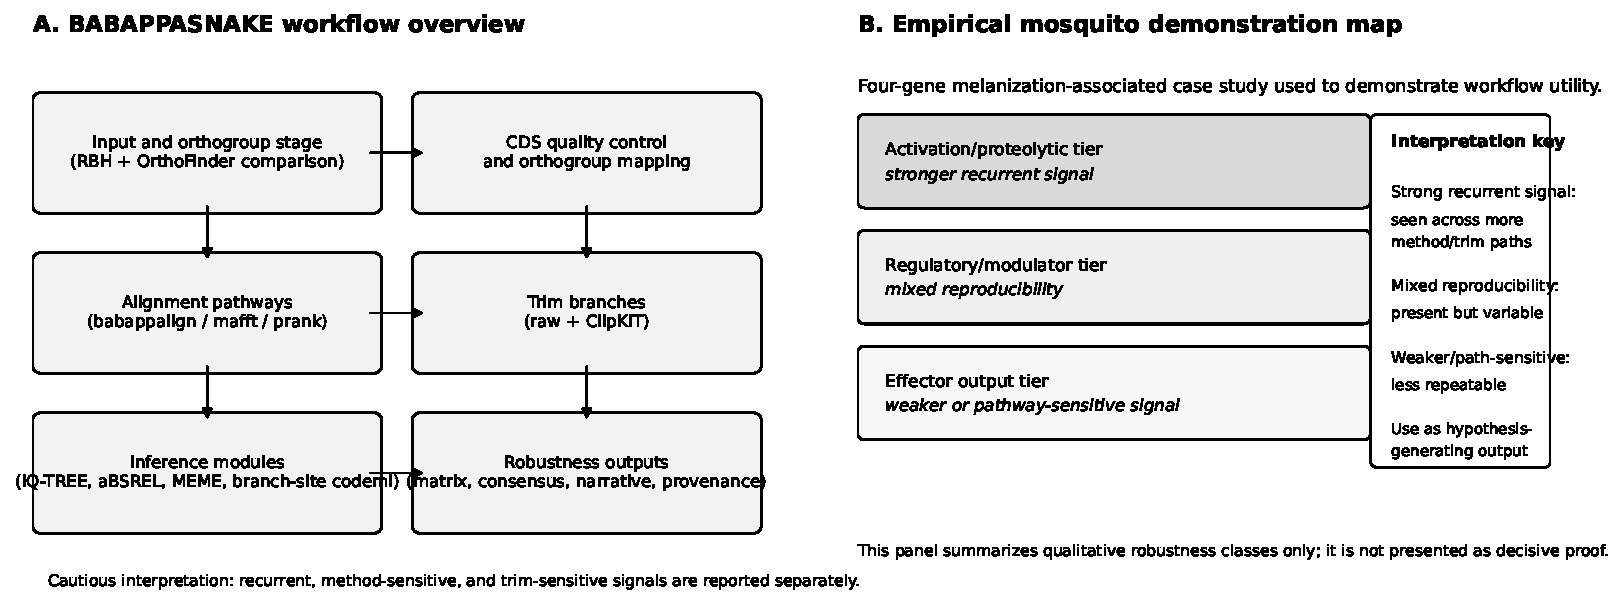
\includegraphics[width=\textwidth]{figures/workflow_case_study_summary.pdf}
  \caption{Method-oriented summary figure. Left: BABAPPASNAKE workflow architecture and output logic. Right: qualitative case-study signal map used as an empirical demonstration (stronger recurrent, mixed, and weaker/path-sensitive classes). The map is presented for robustness-aware interpretation, not as decisive pathway-level proof.}
  \label{fig:workflow_case_demo}
\end{figure}

\section{Results}
\subsection{Workflow behavior and output organization}
In end-to-end execution, BABAPPASNAKE organizes outputs by method and trim state, allowing explicit comparison of signal stability.
The pipeline records orthogroup decisions, pathway-specific inference products, and cross-pathway summaries in a structured hierarchy.
Guided mode additionally supports stepwise execution with safe skip/stop behavior, improving transparency during iterative analyses.

\subsection{Empirical mosquito case-study demonstration}
We applied the workflow to a four-gene mosquito melanization-associated module as a real-data demonstration.
The objective of this analysis was to evaluate practical workflow utility under biologically plausible complexity.

In this demonstration, BABAPPASNAKE recovered a mixture of recurrent and pathway-sensitive patterns across method$\times$trim branches.
Some branch/site signals were recovered in multiple pathways, while others showed method or trim dependence.
The resulting pattern is therefore interpreted as an empirical robustness profile rather than a single definitive biological verdict.

At the pathway-tier level, the demonstration showed directional asymmetry in reproducibility classes (stronger recurrence in some tiers, weaker or less repeatable behavior in others).
Because this manuscript is method-oriented, these observations are treated as hypothesis-generating and as evidence that workflow-level sensitivity reporting is necessary for careful interpretation.

\section{Discussion}
The central contribution of this study is workflow design and implementation: BABAPPASNAKE provides an integrated, reproducible structure for orthogroup-centered episodic selection analysis.
By combining established engines in a single orchestrated pipeline and by exposing robustness outputs across method and trimming choices, the workflow addresses a common practical weakness of fragmented analyses.

The mosquito four-gene analysis demonstrates practical applicability on real data and illustrates how the workflow distinguishes recurring from pathway-sensitive observations.
This use case is informative as an empirical demonstration of utility, but it is not presented as a decisive proof of pathway-level concentration claims.

The reformulation also clarifies interpretation boundaries.
Branch-site follow-up outputs are valuable for prioritization and mechanistic hypothesis generation, yet they remain sensitive to upstream analytical choices.
Explicit robustness reporting helps prevent overstatement and supports transparent downstream reasoning.

\textbf{Limitations and future work.}
This manuscript does not present broad multi-dataset benchmarking against alternative end-to-end pipelines.
Such benchmarking remains an important next step.
Additional future extensions include expanded orthology stress tests, recombination-aware diagnostics, and broader cross-system validation.

\section{Availability, Supplement, and Reproducibility}
\subsection{Code availability}
BABAPPASNAKE source code is available at:
\begin{center}
\url{https://github.com/sinhakrishnendu/babappasnake.git}
\end{center}

\subsection{Data and archive availability}
Case-study outputs are organized as pathway-partitioned run directories with robustness summaries, ASR extraction tables, and provenance JSON files.
The manuscript-level file map is described in the supplementary document.

\subsection{Supplementary information}
Supplementary material provides workflow details, case-study procedural notes, robustness-table organization, and archive/file guidance.

\subsection{Reproducibility statement}
The workflow is implemented as a Snakemake DAG with machine-readable run provenance and reproducibility-oriented summary outputs.
Intermediate artifacts are preserved by stage, method, and trim state to facilitate audit and rerun.

\bibliographystyle{plainnat}
\bibliography{references}

\end{document}
